\documentclass[ALICE,manyauthors]{cernphprep}
\usepackage[comma,square,numbers,sort&compress]{natbib}
\usepackage{hyperref}
\usepackage{lineno}
\usepackage{xspace}
\usepackage[table]{xcolor}
\usepackage{siunitx}
\sisetup{binary-units=true}
\sisetup{load-configurations = abbreviations}
\sisetup{per-mode = symbol}
\DeclareSIUnit\clight{\text{\ensuremath{c}}}
\linenumbers

\input{commands.tex}

\begin{document}

\begin{titlepage}
% the dates below correspond to CERN approval
% please don't touch: EB chairs will take care
\PHyear{XXXX}       % required, will be obtained from CERN
\PHnumber{XXX}      % required, will be obtained from CERN
\PHdate{Day Month}  % required, will be obtained from CERN

%%% Put your own title + short title here:
\title{ALICE upgrades during the LHC long-shutdown 2}
\ShortTitle{ALICE LS2 upgrades}   % appears on left page headers

%%% Do not change the next lines
\Collaboration{ALICE Collaboration\thanks{See Appendix~\ref{app:collab} for the list of collaboration members}}
\ShortAuthor{ALICE Collaboration} % appears on right page headers, do not change

\begin{abstract}
A Large Ion Collider Experiment (ALICE) has been conceived and constructed as a heavy-ion experiment at the LHC. During LHC runs 1 and 2, it has produced a wide range of physics results based using all collision systems available at the LHC.
In order to best exploit new physics opportunities opening up with the upgraded LHC and new detector technologies, the experiment has undergone a major upgrade during the LHC long shutdown 2. This comprises the move to continuous read-out, the complete overhaul of core detectors, as well as a new processing software stack and hardware. 
These improvements will allow us to sample Pb-Pb collisions at rates up to \SI{50}{\kilo\hertz}, while ensuring sensitivity for signals without a triggerable signature.
\end{abstract}
\end{titlepage}

\setcounter{page}{2} %please do not remove this line

\tableofcontents
\listoffigures
\listoftables

\section{Introduction}

A Large Ion Collider Experiment (ALICE) has been proposed and built to study
the properties of the Quark-Gluon Plasma in hadronic collisions at the Large
Hadron Collider at CERN~\cite{Aamodt:2008zz}. The design was driven by the
requirement to cope with the high multiplicities in central \PbPb collisions
and provide a complete reconstruction of the events, including particle
identification over a wide \pt range.

The experimental setup consists of a central barrel contained in a solenoidal
magnet ($B = 0.5~\mathrm{Tesla}$) and a forward muon-system with a dipole magnet
providing $3~\mathrm{Tm}$, see Fig.~\ref{fig:alice_run2}. Until the end of Run~2,
the central barrel contained an Inner Tracking System (ITS) with two layers of
Silicon Pixel Detectors (SPD), two layers of Silicon Drift Detectors (SDD), and
two layers of Silicon Strip Detectors (SSD). In radial direction, it is followed
by a Time Projection Chamber (TPC) covering the radii from 0.5~m to 2.5~m over a
length of 7~m. \dots

\begin{itemize}
\item overview of the detector
  (status as of end of Run 2)
\item barrel tracking
\item detectors for particle identification
\item calorimetry
\item forward physics
\item triggering
\end{itemize}

\begin{figure}
\centering
\includegraphics[width=.7\textwidth]{intro/2017-May-11-ALICE_RUN2_labels_HD}
\caption{Detector setup in Run 2}
\label{fig:alice_run2}
\end{figure}

\subsection{Run1/2 performance highlights (examples)}

cite performance paper~\cite{Abelev:2014ffa}, possibly also detector papers

discuss performance
\begin{itemize}
\item particle identification and relevant detectors
\item secondary vertex resolution
\item data sets (rate/integrated luminosity)
\end{itemize}

Data was recorded throughout the
running of the LHC in Run 1 and 2 exploiting a variety of collision systems and
energies, see Tab.~\ref{tab:datasets}.

\begin{table}
  \centering
  \rowcolors{2}{}{gray!30}
  \begin{tabular}{lrr}
    \multicolumn{1}{c}{system}
    & \multicolumn{1}{c}{$\snn~(\mathrm{\TeV})$}
    & \multicolumn{1}{c}{$L_\mathrm{int}$}\\
    \hline \hline
    \pp & 0.9 & $\sim 200~\mu\mathrm{b}^{-1}$\\
        & 2.76 & $\sim 100~\mathrm{nb}^{-1}$\\
        & 5.02 & $\sim 1.3~\mathrm{pb}^{-1}$\\
        & 7 & $\sim 1.5~\mathrm{pb}^{-1}$\\
        & 8 & $\sim 2.5~\mathrm{pb}^{-1}$\\
        & 13 & $\sim 25~\mathrm{pb}^{-1}$\\
    \pPb{} & 5.02 & $\sim 15 + 3~\mathrm{nb}^{-1}$\\
           & 8.16 & $\sim 25~\mathrm{nb}^{-1}$\\
    \XeXe{} & 5.44 & $\sim 0.3~\mu\mathrm{b}^{-1}$\\
    \PbPb{} & 2.76 & $\sim 75~\mu\mathrm{b}^{-1}$\\
            & 5.02 & $\sim 0.25 + 1~\mathrm{nb}^{-1}$\\
    \hline
  \end{tabular}
  \caption{ALICE datasets from LHC Run 1 and 2}
  \label{tab:datasets}
\end{table}


\section{Upgrade objectives, motivations and goals}
\subsection{physics/performance objectives}
\subsection{requirements on implementations/overall system design}
\begin{itemize}
\item Radiation tolerance/load
\item continuous read-out, no filtering but compression (general description), TF and its related impact on reconstruction, CTP-CRU-FLP-EPN approach, implementation specification (beam, particle load, radiation load)
\end{itemize}


\section{Chip developments (12 p.)}
\input{alpide}
\input{sampa}


\section{Detector systems}
(aim for similar substructure for all detectors)

Some words on setup overview \dots

\begin{figure}
\centering
\includegraphics[width=.5\textwidth]{common/2017-May-11-ALICE_RUN3_labels_HD}
\caption{Overview Run 3}
\label{fig:alice_run3}
\end{figure}

\subsection{ITS (Vito; 10 p.)}

\subsection{MFT (Raphael 5 p.)}

\subsection{TPC (Harry; 10 p.)}



\subsection{Fast Interaction Trigger (FIT)}

\begin{figure}[htbp]
\begin{center}
\includegraphics[width=0.8\linewidth]{fit/f40Fit3dCompleteTable.png}
\caption{View of FIT detectors illustrating the relative sizes of each component.  From left, FDD-A, FT0-A, FV0, FT0-C, FDD-C.  Note that FT0-A and FV0 have a common mechanical support. FT0-A is the small quadrangular structure in the centre of the large, circular FV0 support. Note that all are planar with the exception of FT0-C which has a concave shape centered on the IP.  The inset table lists the distance from the IP and the pseudorapidity coverage for each component.  }
\label{FITschematic}
\end{center}
\end{figure}

The Fast Interaction Trigger (FIT)\cite{Trzaska:2017reu} serves as an interaction trigger, online luminometer, initial indicator of the vertex position, and the forward multiplicity counter. In the offline mode it provides the precise collision time for the TOF-based particle identification, yields the centrality and interaction plane, and measures cross sections of diffractive processes. To deliver the required functionality, the active elements of FIT use three different detector technologies grouped into five arrays, as shown in fig.~\ref{FITschematic}. Their distance from the IP and their pseudorapidity coverage are displayed in the inset table in .~\ref{FITschematic}. The naming convention relates to the similar ALICE detectors used during Run 2. FT0 is the successor of T0~\cite{Bondila:2005}; FV0, of V0~\cite{V0performance:2014}; and FDD, of AD~\cite{broz:2020mb}. The main reason for the upgrade is the increased luminosity and interaction rate~\cite{Trzaska:2020zzl}, which can reach 1 MHz in proton$-$proton (pp) and 50 kHz in Pb$-$Pb collisions during LHC Runs 3 and 4. To cope with the increased interaction rate and to enable continuous readout, a new fast electronics and readout system~\cite{Finogeev:2020qkf} have been designed and implemented for all FIT subdetectors.

%In order to maintain the physics performance of the detectors replaced by FIT, FT0 is optimized to provide very good timing and a highly efficient fast multiplicity trigger, FV0 allows for the measurement of multiplicity as a function of pseudorapidity and azimuthal angle, and FDD's  coverage at small angles with respect to the beam gives access to measurements of diffractive processes. FT0 and FDD have arrays on either side of the nominal interaction point; FV0, due to severe space constraints, is only on the A side. 


 \subsubsection{FT0}
 
The FT0 consists of two
arrays, FT0-A and FT0-C, of  quartz Cherenkov radiators optically coupled to Photonis XP85002/FIT-Q microchannel
plate-based photomultipliers (MCP), which are factory customized versions of the Planacon XP85012. The modification is a new back-plane designed specifically for FT0 grouping the 64 anodes into 4 outputs. The 4 independent outputs deliver signals from 4 optically isolated 2\,cm thick  $2.65\times 2.65 \,\rm{cm}^2$  quartz radiators.  The signal path from each anode is the same length to improve the timing properties of the system.  This segmentation allows for providing the granularity for measurements of  multiplicity in central Pb$-$Pb collisions and has very good coverage of the solid angle subtended by the detector.  The intrinsic time resolution of each quadrant is  $\sigma_{\rm t} \approx 13\, {\rm ps}$ \cite{Melikyan:2020owp}. Accounting for signal deterioration along the 30 m long signal cables and processing by the 
front-end electronics, the achieved one-MIP time resolution of FT0 is about 25\,ps.  
The efficiency of the Minimum Bias trigger for pp collisions is  $\geq 98\%$ for the OR of the two sides and  $\geq 77\%$ for coincidences between FT0-A and FT0-C.
%\begin{figure}[htbp]
%\begin{center}
%\includegraphics{FT0C.jpg}
%\caption{Support structure for the FT0-C.}
%\label{FT0Cfig}
%\end{center}
%\end{figure}


FT0-A, located 3.3 m from the IP has 24 modules and thus 96 individual readout channels.
Due to the close proximity to the IP, the FT0-C support has a convex shape (as seen from the IP) positioning all 28 MCPs such that each of the 112 quartz radiators is 84 cm from the nominal IP.
 
\subsubsection{FV0}
FV0 is a large, segmented scintillator disk with a novel light collection scheme \cite{grabski2019new} assuring short pulses, single MIP time resolution of $\approx 200\, \rm{ps}$  , and a very uniform response across the entire detection surface. The active element of FV0 is a 4 cm thick EJ-204 plastic scintillator divided into 5 concentric rings of equal pseudorapidity coverage. The outer diameter of the largest ring is 144 cm and the inner diameter of the smallest is 8 cm. The 4 inner rings are subdivided into 8 sectors of 45 degrees each while the outermost ring, due to its large area, has 16 sectors. A grid of equal-length, clear Ashai fibres is attached to the back side (as viewed from the IP) of the scintillator as can be seen in fig.~\ref{FV0fig} At the other end, the fibres from each sector form a bundle and are optically coupled to Hamamatsu R5924-70 PMTs. This way, the 48 sectors of FV0 deliver 48 independent readout channels. This segmentation, combined with the information from the other forward detectors, is sufficient to yield the required centrality and event plane resolution. Together with FT0, FV0 provides the needed input to generate Minimum Bias and Multiplicity trigger at the LM (Level Minus one) level. Having the total latency below 425\,ns, this is the fastest trigger in ALICE. In addition, the FV0 monitors LHC background conditions and luminosity. 

\begin{figure}[htbp]
\begin{center}
\includegraphics[width=0.9\linewidth]{fit/FV0_crossSection.jpg}
\caption{ Photograph of one half of the FV0. The optical fibers connect the scntillators to the PMTs on the rim of the support structure, the black structure seen here. The center wall has been removed to show the scintillator, surface matrix structure, and optical fibers.}
\label{FV0fig}
\end{center}
\end{figure}


\subsubsection{FDD}
The FDD \cite{Rojastorres} comprises  two nearly identical arrays, FDD-A and FDD-C, surrounding the beam pipe on opposite sides of the IP.  Each array consists of eight rectangular pads, $216 \times 181 \times 25\, \rm{mm}^3$ BC420 scintillator. The pads are assembled as  two overlapping layers of four sectors each. To make clearance for the beam pipe, a quadrant was removed from the innermost corner of each scintillator plate. The diameter of the removed quadrant on the FDD-A scintillators is 124 mm and 74 mm on the FDD-C as illustrated in fig.~\ref{FITschematic}. Each pad has two wavelengths shifting (WLS)
bars attached to the opposite sides of the scintillator. Clear optical fibres carry the light
from the WLS to H8409-70 PMTs. There are 8 independent FDD channels on each side of the IP.

Benefitting from the much improved ITS capability of heavy flavour tagging in the central barrel, the FDD contributes to the measurements of diffractive cross sections and studies of ultra-peripheral collisions. In pp collisions, the main physics objectives of the FDD are the studies of centrally produced exclusive states, measurements of cross sections for single and double diffraction, and inelastic processes at the new LHC centre of mass energy of 14 TeV. In Pb$-$Pb and p$-$Pb collisions, the FDD provides an independent measurement of centrality in an intermediate pseudorapidity range between the ITS and the ZDC and contributes to the selection of ultra-peripheral collisions. In the online mode, the FDD is used to monitor beam quality and to reject beam-gas events. 


\subsubsection{Electronics and readout scheme}

\begin{figure}[htbp]
\begin{center}
\includegraphics[width=0.9\linewidth]{fit/FIT_data_processing.png}
\caption{Schematic diagram of the FIT readout electronics. }
\label{default}
\end{center}
\end{figure}
All three subsystems of FIT use the same front-end and readout electronics based on just two custom-designed modules: a Processing Module (PM) and a Trigger and Clock Module (TCM). One PM provides 12 independent inputs. Each sub-detector has only one TCM while the number of PMs is determined by the number of channels. Each PM is connected to the dedicated TCM via an HDMI cable to transmit "pre-trigger" data, slow-control data and LHC clock distribution. The commands, configuration data, and status data are sent from the ALICE control system to the TCMs via a 1 Gb Ethernet optical link using an IPbus (UDP
based protocol) \cite{Finogeev:2020qkf}. The triggers and the measured event rates for the luminosity
measurements are transmitted from the TCMs via the same connection. The PMs are
configured from TCMs via an HDMI SPI connection. The PMs and TCMs are connected
to the ALICE DAQ with GBT links. FIT delivers the produced trigger signals to the Central Trigger System.
 
Laser pulses are used for time and amplitude calibration, as well as monitoring of ageing and radiation damage of the FIT detectors.


\subsection{Muon System}

The forward muon arm has been described in ~\cite{Aamodt:2008zz} . It consists of a
composite absorber ($\sim 10\ \lambda_{int}$), made with layers of
both high- and low-Z materials starting 90 cm from the mean
interaction point, a large dipole magnet with a 3 Tm integrated field
placed outside the L3 barrel magnet, and ten planes of very thin, high
granularity, cathode pad tracking stations. A second muon filter
($\sim 7\ \lambda_{int}$ of iron) at the end of the spectrometer and
four planes of Resistive Plate Chambers are used for muon
identification. The spectrometer is shielded by a dense conical
absorber tube, of about 60 cm outer diameter, which protects the
chambers from secondary particles created in the beam pipe.

The increase of luminosity of the LHC after LS2 requires an upgrade of
the front-end and read-out electronics on both muon
tracking and muon identifier subsystems.


\subsubsection{Muon Tracking}

The Muon Tracking Chambers (MCH)~\cite{Aamodt:2008zz} was operated
during LHC run~1 and run~2. It is based on 156 multi-wire proportional
chambers with cathode pad readout, the so called Cathode Pad Chambers with more than
one million electronic channels. 
The system consists of 5 tracking stations, each of which is composed of 2
chambers. Because of the different sizes of the stations, (ranging from few square metres for station 1 to more than 30 m$^{2}$  for station 5) two different designs were adopted. The first two stations are based on a quadrant structure ~\cite{Peyre}, with the readout
  electronics distributed on their surface (see Figure ~\ref{quad+slat} (Left) ). Four independent quadrants constitute one chamber. For the larger stations (3 to 5), a slat architecture ~\cite{Cicalo} was chosen (see Fig. ~\ref{quad+slat} (Right)). The maximum
  size of a slat is 40 $\times$ 240 cm$^{2}$ and the electronics are mounted on the top and bottom part of
  each slat. Slats are mounted on a support to constitute one
  half-chamber. One half-chamber consists of 9 slats for station 3,
  and 13 slats for stations 4 and 5. The tracking system
  covers a total area of about 100 m$^{2}$. 

\begin{figure}[h]
  \centering
  \includegraphics[width=.45\textwidth]{mch/quadrant.png}
  \hspace{0.05\textwidth}
  \includegraphics[width=.45\textwidth]{mch/slat.png}
   \caption[Tracking system layout]{Left: Layout of station 2 of the tracking system; the readout electronics is distributed on the surface of a quadrant. Right: Layout of stations 4 and 5 of the tracking system; the readout electronics are mounted along the top and bottom edge of the slats.}
  \label{quad+slat}
\end{figure}

Due to the increase of luminosity of the LHC after LS2, the front-end
and the readout electronics have been upgraded, keeping the detectors
unchanged.

The electronics can run either in trigger or in our default dead time free continuous
mode. The data flow readout scheme is shown in
Fig.~\ref{readoutscheme}. The Front-end Cards (FEC) send continuously words through an electrical link at 80 Mbit/s to the SOLAR
read-out board which connects to the Concentrator Readout Unit (CRU)
through GBT optical link at 3.2 Gbits/s.

\begin{figure}[h]
  \centering
  \includegraphics[width=1\textwidth]{mch/readoutscheme.pdf}
     \caption[Tracking readout scheme]{ The Muon Tracking readout scheme}
  \label{readoutscheme}
\end{figure}

\paragraph{The DualSAMPA front-end electronic cards\\}

The front-end electronic cards, called DualSAMPA, host 2 chained SAMPA chips (
see chapter 3.2) of 32
channels each and 3 low voltage regulators. Since the detectors are not
changed, the dimensions and the layout of the connectors for the DualSAMPA cards on the
electronic PCBs remain the same as for the previous FEC. Moreover, two
types of cards were produced, each with the same functionalities but with
different dimensions to cope with the two detector types, quadrant and
slat (see Fig.~\ref{dualsampa}).

\begin{figure}[h]
  \centering
  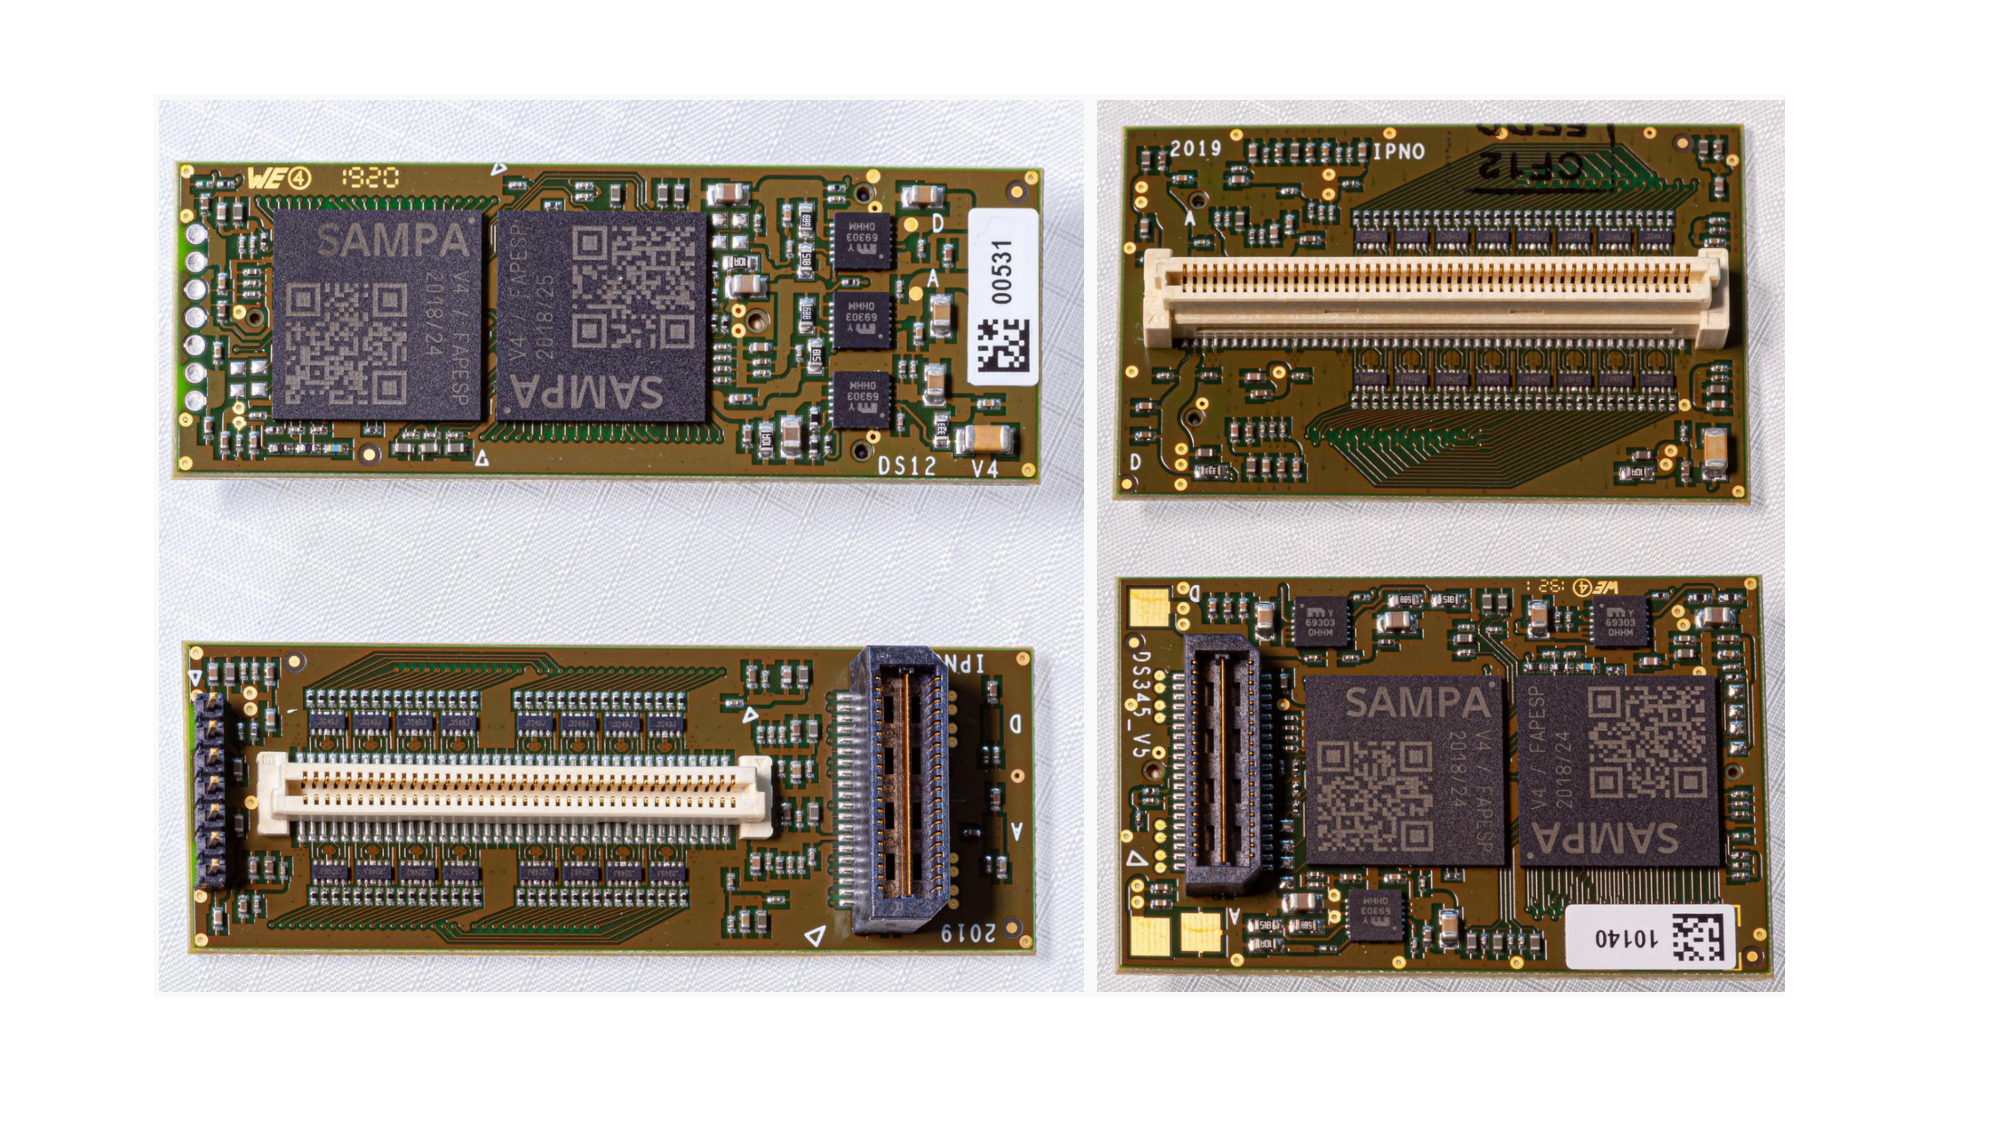
\includegraphics[width=1\textwidth,height=8cm]{mch/dualsampa.pdf}
     \caption[DualSAMPA]{ The two geometries of the DualSAMPA boards,
       with the white connector plug socket on PCB and on the
       other side the black connector connecting to the electrical link. }
  \label{dualsampa}
\end{figure}


Out of the 19300 DualSAMPA produced (11000 DS345 for slats of stations 3,4 and
5 and 8300 DS12 for quadrants of stations 1 and 2), 16900 are
installed in the cavern (9700 DS345, 7200 DS12).

\paragraph{The readout electronic FLEX links and large electronic PCBs\\}

The link between the DualSAMPA and the readout cards consists of a
flexible circuit (FLEX) and a flat ribbon cable for the slats while a
large electronic PCB and a flat ribbon cable is used for the quadrants (see
Figs.~\ref{flex+pcb}(Left) and ~\ref{flex+pcb} (Right)).

\begin{figure}[h]
  \centering
  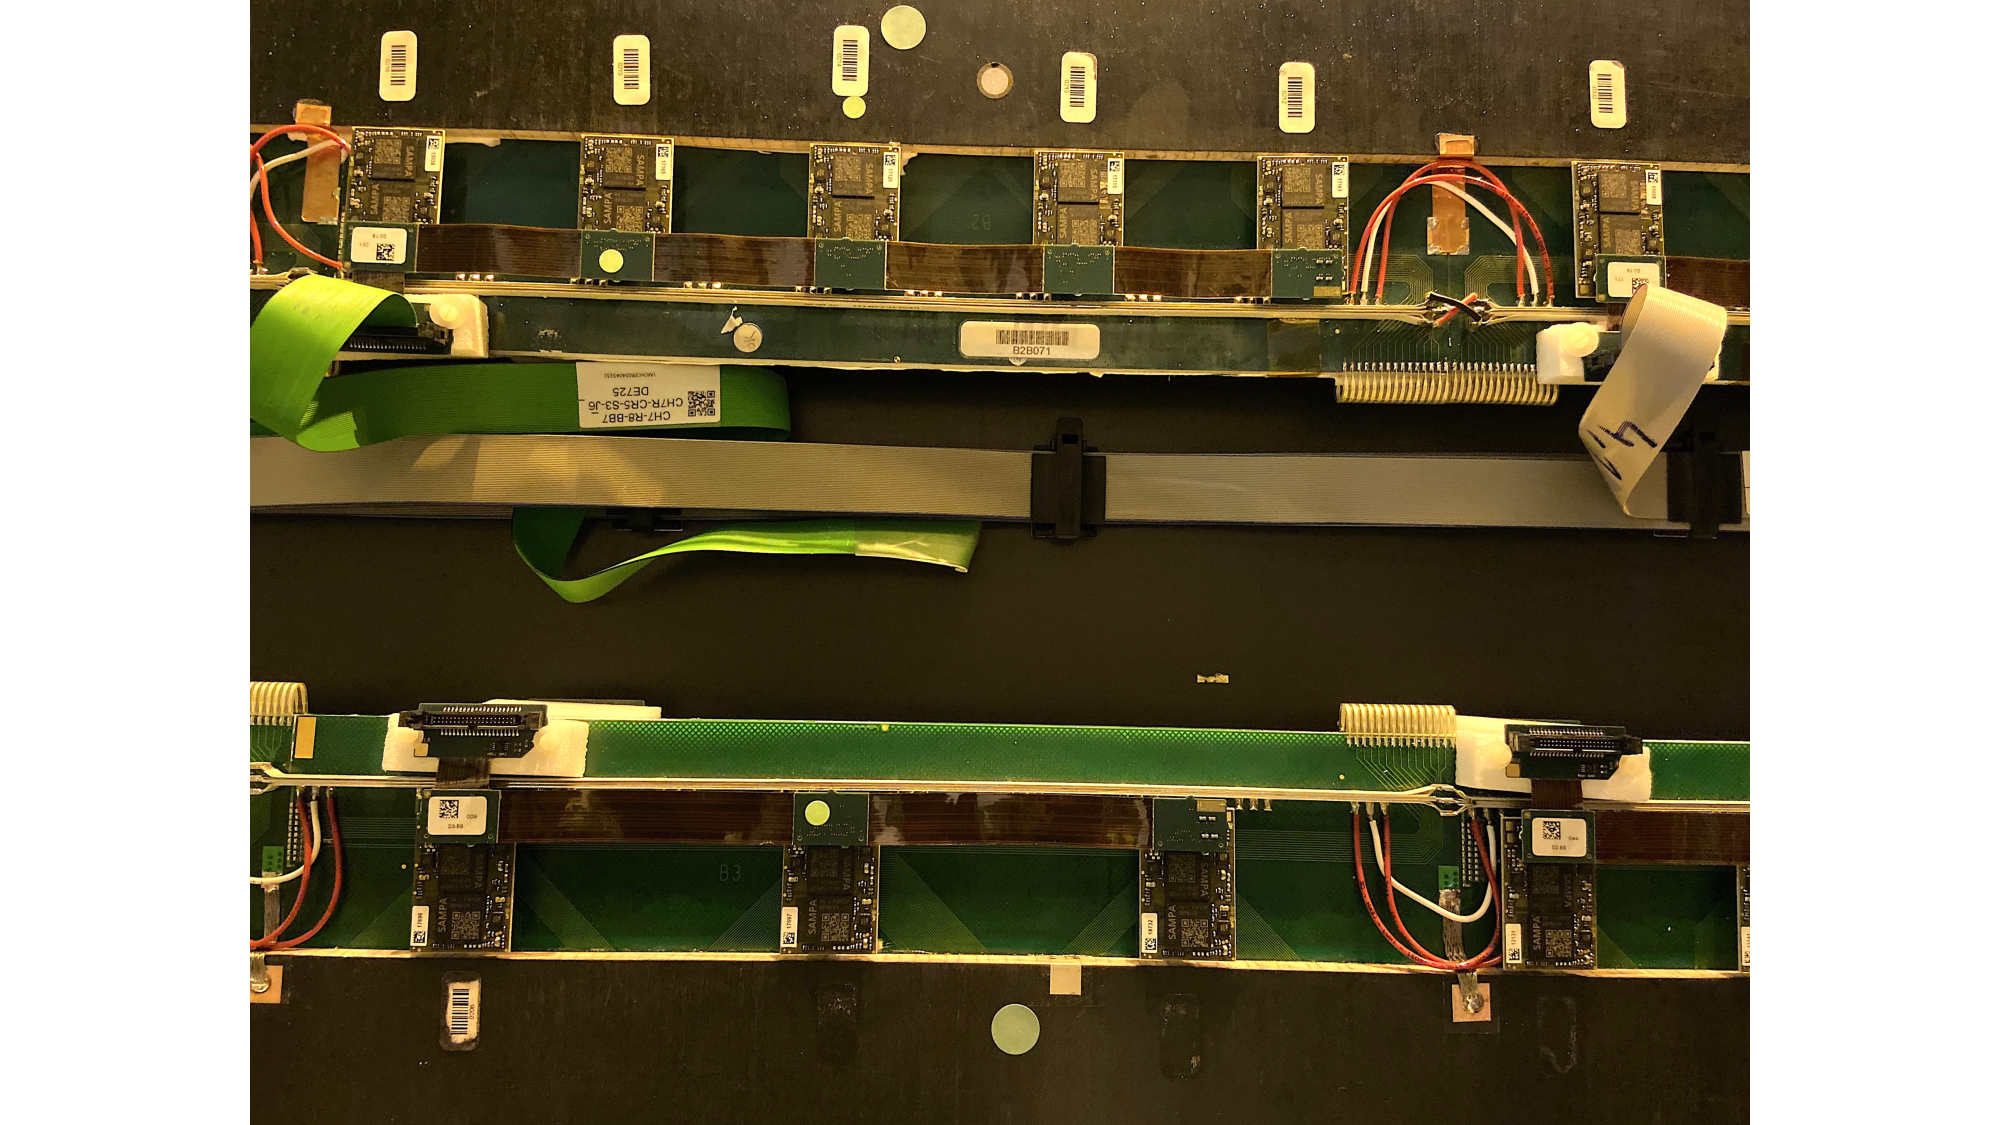
\includegraphics[width=.45\textwidth,height=5cm]{mch/flex.png}
  \hspace{0.05\textwidth}
  \includegraphics[width=.45\textwidth,height=5cm]{mch/largepcb.png}
   \caption[Electronic links]{Left:Flex mounted on a slat connecting 5
     DualSAMPA cards linking through a green flat ribbon cable with the readout
     board. Right:Large electronic PCBs covering the surface of a quadrant.}
  \label{flex+pcb}
\end{figure}

Each DualSAMPA has dedicated data and clock lines while the
trigger lines are daisy chained to feed up to 5 DualSAMPA (see
Fig.~\ref{flexscheme}). A I2C line allows to address up to 5
DualSAMPA. An active buffer was added to the I2C line to insure a
good signal integrity.

More than 3000 FLEX were produced, of 24 different types depending on the number of DualSAMPA
to address, the geometry and pad density; among them 2760 were
installed.
 
\begin{figure}[h]
  \centering
  \includegraphics[width=0.8\textwidth, height= 4cm]{mch/flexscheme.png}
     \caption[FLEX scheme]{ The FLEX scheme}
  \label{flexscheme}
\end{figure}



\paragraph{The SOLAR readout cards\\}
Each FLEX/ribbon cable is plugged into one of the 8 ports of the SOLAR readout
board, allowing this latter to read out up to 40 DualSAMPA boards (see
Fig.~\ref{solarscheme}). The GBTx chip of the SOLAR
board acts as a deserializer of the  signal coming from the DualSAMPA
and a serializer to send the signals from the different FEC to the CRU through GBT optical
links. The SOLAR board hosts also a GBT-SCA chip handling the 8 I2C
command/control lines, one optical transmitter/receiver VTRx and 2
DC/DC FEAST converters. 
 
\begin{figure}[h]
  \centering
  \includegraphics[width=1\textwidth]{mch/solarscheme.png}
     \caption[SOLAR scheme]{ The SOLAR scheme}
  \label{solarscheme}
\end{figure}

The 624 boards produced are placed in 112 custom SOLAR crates, each
one hosting up to 6 boards.


\paragraph{The data flow from SAMPA to the CRU User Logic\\}
In the SAMPA chip, the signal of each electronic channel is amplified with a ~4mV/fC gain,
waveformed with a shaping time of 300 ns, then sampled and digitized at 10 MHz in
a 10-bits ADC and is finally digitally processed with a baseline
correction and a zero-suppression before being formatted. The SAMPA format
consists of data samples from a signal waveform with its time stamp and
size together with a header containing mainly the bunch crossing number, the SAMPA
address and the channel address of the SAMPA chip.

 The signals of the 64 channels of
the two-chained SAMPA chips of a FEC are serialized at 80
Mbits/s (2bits at 40 MHz). The first port of the SOLAR board handles
the first 2 bits of the first DualSAMPA while the second port takes care of the 2 bits of
the second DualSAMPA and so on up linking all 40 ports whihc results in a 4.2
Gbits/s data optical transmission to one input of a CRU. The
electrical and optical links are always sending words, whatever the
type of information (physics data, synchronisation (SYNCH), ...). 

The MCH CRU User Logic (UL) receives data from the 24 GBT links (see description of the CRU in
chapter 6.3), each one handling 40 DualSAMPA channels. For each GBT
link, the UL deserializes the 80 bits, forms the SAMPA
words, remove the SYNCH words and inserts error checks and
condition. The 64 bits SAMPA words contain the payload, the GBT
link identifier, the DualSAMPA channel identifier, and error bits. The
UL then embeds the TTC signals into the stream, constructs
the RDH (Redaout Data Header) and transmits words of 256 bits to the FLP (Front Level
Processor) (see Fig. ~\ref{dataflow} and~\ref{cru-ul}).

\begin{figure}[h]
  \centering
  \includegraphics[width=0.7\textwidth,height=3cm]{mch/dataflow.png}
     \caption[Data flow]{Data flow scheme}
  \label{dataflow}
\end{figure}

\begin{figure}[h]
  \centering
  \includegraphics[width=1\textwidth]{mch/cru-ul.png}
     \caption[CRU Scheme]{CRU scheme}
  \label{cru-ul}
\end{figure}

The $O^2$ processes, carried out on FLPs or/and EPN,  will perfom the decoding of the data
format received from the CRU, the pre-clustering, clustering and tracking. These
will also run the simulations.
During data taking the Quality Control (QC) processes data samples for detector performances
monitoring.



\input{mid}
\subsection{TRD}

The construction, operation and performance of the Transition Radiation Detector (TRD) is presented in Ref. \cite{Acharya:2017lco}. Here we focus on modifications implemented for the high rate running in LHC Runs 3 and 4.

\subsubsection{HV distribution and common mode}

During TRD operation in Run 1 and Run 2, a number of anode and drift channels of individual chambers developed high currents and were eventually not operational any more. The built-in decoupling capacitors in the on-detector HV distribution system were considered probable candidates given the experience of the TPC and from the repair of supermodule (SM) 17 during the long shutdown (LS) 2. At that point, construction of the TRD was still ongoing and the last 4 supermodules were built without the biggest capacitors in the HV distribution (4.7 nF). In total, until the end of Run 2, 70 anode channels and 20 drift channels were taken out of operation from a total of 522 chambers installed in 18 SMs.

\begin{figure}[hbt]
    \centering
    \includegraphics[width=0.5\textwidth]{trd/TRD_front_repaired_label_V2.pdf}
    \caption{The status of SMs concerning capacitors in the HV distribution.}
    \label{fig:TRD_status}
\end{figure}

The HV distribution with the decoupling capacitors on filter boards is mounted directly on each chamber and therefore encased in the hull of the SMs. It was possible to access these locations via milling cut-outs into the casing and removing the top cover to give access to all 30 chambers in a SM. 
Each anode as well as drift channel hold a 4.7 nF capacitor; the anode wire plane is segmented in 8 or 6 sectors of two pad rows each, decoupled from each other by a 2.2 nF capacitor. Measurements of capacitors that were removed confirmed the reason for the HV failures, explaining the observed issues. Most of the problems could be traced to failing 4.7 nF capacitors but it was found that also a small fraction (in the percent range) of the 2.2 nF capacitors had failed. Therefore, all 4.7 nF and 2.2 nF capacitors on the filter boards were removed from a total of 9 TRD SMs. This number was determined by the turn around time of SM deinstallation from the space frame of ALICE, repair, test and reinstallation during the first year of LS2. Before reinstallation of each SM, long-term HV, LV, cooling and readout tests were performed to ensure proper detector operation.
It turned out that 96\% (80 out of 83 not operational chambers) in the 9 SMs could be restored. 
Figure \ref{fig:TRD_status} displays the configuration of the individual SMs in terms of installed decoupling capacitors. Based on experience we estimate that by the end of Run 4 MM chambers in the 4 SMs labelled as unchanged in the figure and NN chambers in the 5 SMs already built without the 4.7 nF capacitors will develop failures. Therefore good tracking capability in all sectors is ensured for the entire planned period of operation. 

As the capacitors were meant to buffer high charge deposits in the chambers, their removal results in larger induced common-mode signals on readout pads in the same high-voltage segment. The measured common-mode signal is shown in Figure \ref{fig:common_mode_ph} and is about three times larger than with the capacitors in place, consistent with the expectation from the remaining capacitance of the readout chamber.
This effect will be corrected in software based on the measured local charge deposit.

\begin{figure}
    \centering
    \includegraphics[width=0.6\textwidth]{trd/trd_common_mode.pdf}
    \caption{Induced common-mode signal with and without capacitors for the anode HV. The baseline of pads in the same high-voltage segment as a cosmic ray particle with an integrated signal between 10\,000 and 12\,500 ADC counts is shown before (red) and after (blue) the removal of the capacitors. For comparision, the baseline from pads in high-voltage segment without hits is shown in green.}
    \label{fig:common_mode_ph}
\end{figure}
 
\subsubsection{Readout}

The readout chain has been optimised in the past for a high event inspection rate at LM level with a fast calculation of the L1 trigger contribution (LM tracklet data readout time < \SI{8}{\micro \second} , L1 decision time < \SI{6}{\micro \second}), while transferring large, high resolution raw data for events accepted beyond the L1 level (L1 raw data readout time $\approx$ \SI{300}{\micro \second}). In Run 3, the L1 trigger functionality is no longer required and the detector must provide readout rates as high as feasible while writing all events to permanent storage. No data shall be discarded in the readout chain and the fraction of recorded events in \SI{1}{\mega \hertz} interaction rate pp collisions or \SI{50}{\kilo \hertz} Pb--Pb shall be maximised.

The applied solution is presented in the following sections. Simulations confirm that it enables collecting more than  $\SI{70}{\percent}$ of events in a \SI{50}{\kilo \hertz} interaction rate Pb--Pb running scenario.

\subsubsection{Optimisation of the existing FEE}

In order to achieve a high event readout rate in Run 3, the tracklet readout mode, which has been used to find fast L1 trigger contributions in Run 2, will be used.
The maximum data volume per LM trigger and per Multi Chip Module (MCM) is 4 words of 32 bits each. The usage of the available bits is no longer optimised for triggering, but for physics analysis.

Previously, each MCM processed and transmitted up to 4 tracklets, each as a 32-bit word.
However, even in the most central Pb--Pb events a track density of 4 tracklets per MCM has been rarely reached. Therefore, only 3 tracklets per MCM are allowed in the Run 3 data format. The estimated fraction of tracklets lost by this measure in central Pb--Pb events is below 1\%.
The freed-up 32 bit word is used as a header to store position information about the MCM and 8 bit of PID information per tracklet. It is followed by 1 to 3 32-bit tracklet words that store the position within the MCM, slope and additional 12 bits of PID information of the tracklet. The details are shown in Table \ref{tbl:tracklet:format}.
The PID information per reconstructed tracklet will increase from 8 to 20 bits, which will be used to store charge information from three time slices with 6 or 7 bit dynamic range each. Simulations have shown that the expected performance with this data format is similar to an offline analysis with the same number of time slices. The tracklet position and slope will also be stored with higher precision than in previous runs. 
 
 In previous runs, a preselection cut based on the tracklet inclination has been applied to tracklets in the FEE. This cut is lifted in order to avoid any possibble bias in the collected physics data.
        
In Run 3, the TRD uses a Physics trigger sent by the CTP at LM latency. In addition, the TRD supports a new trigger type, called calibration trigger. The calibration trigger, also sent at LM latency, enables the shipping of Physics data and, additionally, the full raw data. This allows to trigger a full readout for a small fraction of events, facilitating detector calibration. Apart from that, the calibration trigger is interpreted by the FEE as a command to reload its configuration parameters from hamming protected memory areas. This is a precaution measure and mitigates the impact of Single Event Upsets (SEUs) on data taking, sporadically observed on some isolated half chambers as Link Monitor Errors (LMEs) in previous Runs.

\begin{table}[!ht]
    \label{tab:trackletformat}
    \begin{tabular}{lc}
         Header & 
        \bitpattern[startBit=31]
        {1}[1] {padrow}[4] {col}[2] {HPID2}[8] {HPID1}[8] {HPID0}[8] {1}[1]/
         \\
        Payload (1-3x)
        &
        \bitpattern[startBit=31] {position}[11] {LPID}[12] {slope}[8] 0[1]/
    \end{tabular}
  
  \caption[Tracklet data format]{TRD tracklet data format. Each MCM that has reconstructed at least one tracklet will send a header with shared coordinate information and 8 bits of PID information per tracklet. For each reconstructed tracklet, one additional payload word with additional position and PID information as well as the reconstructed tracklet angle (slope) will be stored.}
  \label{tbl:tracklet:format}
\end{table}


\subsubsection{Common Readout Unit (CRU)}

For Run 3, the Global Tracking Unit (GTU) is replaced by CRUs. The CRUs receive the data directly from the FEE via 1080 optical links. Every CRU provides 30 link inputs, implying that in total 36 CRUs are in use. They are housed in 12 First Level Processors (FLPs).

The FPGA firmware on the CRU has been developed in a joint effort between O2 and TRD. It controls the readout process of the detector, receives, buffers and formats the data for the O2 system. All CRUs are connected to the LTU on the CTP side to receive trigger information and to signal a detector busy status to the CTP. Each CRU determines an individual busy status contribution depending on the status of the readout of the connected FEE links. The CTP combines the busy status contributions from all CRUs in order to determine a global busy status of the detector.

The O2 system performs  a deeper level reformatting and data compression before the data is written to permanent storage.
The following points describe sequentially the process of acquiring an event explaining the role of the the CRU and the interactions with other readout components:

\begin{enumerate}
    \item CTP sends a trigger at LM latency (Physics or calibration) via the LTU to the FEE and to the CRUs in parallel. The trigger to the FEE is shipped via the TTC network. The trigger to the CRU is sent via 9 newly set up trigger distribution networks. They use the new Trigger and Timing Control via TTC-PON technology. A large number of networks, 9, is necessary to achieve minimum latency. The CRUs store all information from the received trigger message (e.g. orbit id, bunch crossing id, etc.) in internal buffers.
    
    \item Upon the arrival of the trigger, the FEE begins recording the data while primary charge drifts towards the anode region. Each CRU receives the trigger at approximately the same time and internally opens a time window within which it is waiting for the input links to send all the acquired data. The timeout is programmable. In addition, each CRU generates its busy status contribution and sends it to the CTP. The TTC-PON upstream communication feature is used to transmit the busy status signal. This prevents the CTP from sending any other trigger as long as any CRU contributes an active busy contribution in order to avoid confusion of the FEE state machines.
    
    \item When the FEE has acquired and processed the data, it starts shipping it via TRD custom optical links based on 8b10b encoding. At the end of the transmission, the FEE appends specific end markers. The CRUs record the data received on all input links.
    In case no data end marker is recognised by the CRU within the programmable timeout or data words are received outside the data expectation window, the CRU marks the concerned link as erroneous (LME) and excludes it from data taking until a manual or automated recovery takes place. The CRU stores all received data in large internal data buffers whose size is sufficient to hold even entire calibration data events at maximum measurable multiplicity. When the CRU has confirmed the reception of end makers on all active links or the timeouts have been reached, the CRU releases its busy status contribution. The CTP considers the detector as busy until all 36 CRUs have released their busy contribution. 
    
    \item Once the detector side of the event acquisition is finalised and the data is stored in internal buffers, the CRU is ready to acquire the next event, while at the same time reformatting the buffered data and shipping it to O2. The CRU packs the data into packets of a maximum size of \SI{8}{\kilo B} and equips these packets with Raw Data Headers (RDHs). In addition, TRD-customised headers are inserted into the data stream. The headers contain various information, including the trigger timestamp information, in order to link the acquired data to other detector data during reconstruction.
    
    \end{enumerate}

\subsubsection{DCS}

A special feature of the upgraded TRD DCS system is that the readout chain status of all half chambers is made available to the DCS system by the CRU. The CRU firmware contains a dedicated error state machine for all half chambers. If a connected half chamber shows a misbehavior, which can be detected at the CRU level, the corresponding state machine enters an error state. This error state is stored in a dedicated CRU register, which is read by the DCS system via the ALFRED \cite{Jadlovsky:ICALEPCS2017-THPHA208} architecture. The obtained status of all half chambers is displayed on a dedicated DCS panel in order to monitor LMEs.

\subsubsection{Standalone tracking}
\label{sec:TRD_stand_alone_tracking}
A stand alone tracking algorithm for the TRD was implemented using a Kalman filter approach. The seeding is using the direction and position information of any two TRD tracklets. The track reconstruction efficiency and transverse momentum resolution was determined via matching to tracks from the Time Projection Chamber (TPC).
For the TRD standalone tracking and the current tracklets (without pad tilt correction) a momentum resolution of about 9\% for 500 MeV/$c$ particles was achieved for the case of 6 tracklets in the fit. By including the primary vertex information as an additional constraint, a momentum resolution better than 4\% was achieved. The TRD stand alone tracking algorithm was so far already used to identify and study photon conversions and nuclear interactions in front of and within the TRD. It will also be used for the TRD drift velocity calibration in Run 3.

\subsubsection{Calibration}

The Run 3 TRD calibration procedure is similar to the one employed before, except for the drift velocity calibration, which will be based on a new development. The angle between a TRD tracklet and the corresponding TRD standalone track, $\Delta \alpha$, is measured as a function of the track impact angle for each chamber. 
A model which includes as free parameters the effective drift velocity $v_{D}^{eff}$ and the Lorentz angle $\alpha_{L}$ is used to fit the distributions. An example for detector 7 is depicted in Fig. \ref{fig:calibrate_5} (left). The effective drift velocity is compensating the ion tail effect which is systematically changing the tracklet angle. The physical true drift velocity $v^{true}_{D}$ is about 35\% larger than $v_{D}^{eff}$. A closure test with 50k events was performed using Run 2 data and the new $v_{D}^{eff}$ parameters. The average angular difference between tracklets and TRD track is zero, as shown in Fig. \ref{fig:calibrate_5} (right).

\begin{figure}[htb]
  \centering
    \includegraphics[width=0.42\linewidth]{Delta_alpha_vs_impact_angle.png}
    \includegraphics[width=0.45\linewidth]{Delta_alpha_after_calib_V4.png}
  \caption{Left: $\Delta\alpha$ versus impact angle for a typical TRD chamber in Run 2, having a fixed uncalibrated drift velocity. The upper values refer to the Run 2 calibration procedure, the lower ones to the new calibration scheme. Right: Average $\Delta\alpha$ versus impact angle distribution for all TRD detectors after the calibration was applied. The red band shows the RMS of the distribution.}
  \label{fig:calibrate_5}
  \end{figure}

About 100k MB p--Pb equivalent events are needed for an update of the calibration parameters. This is similar to what was used in the past in Run 2 with about 600-3000 good tracklets per chamber. The seeding and Kalman filter procedures need on average 10 ms per p--Pb event. In total, not more than 20 minutes for one update of the calibration parameters is needed on a single CPU core. 
The time consuming tracking part will be parallelized.

\subsubsection{Quality Control}

The O2 system for the TRD will use the Quality Control (QC) framework to consolidate the online Data Quality Monitoring (DQM) and offline Quality Assurance (QA) into a single system. The QC system consists of tasks that are running in various parts of the O2 system and produce QC objects, mostly in the form of histograms.

\begin{itemize}

    \item Raw data format. The data arriving from the FEE via the CRU is validated, allowing to detect disabled or malfunctioning parts in the readout tree or SEUs in the FEE. 
    
    \item Zero-suppressed ADC data from all calibration events will be analyzed to reconstruct the average, time-dependent signal shape for each of the 522 readout chambers. These histograms are a versatile low-level monitoring tool for many aspects of the operation of the TRD, including trigger timing, drift velocity and gas gain.
    
    \item Tracklets from a small fraction of events complement the ADC data QC and monitor the local reconstruction of track segments in the FEE of each chamber.
    
    \item Tracking QC will run during synchronous and asynchronous reconstruction and monitor the efficiency at the tracklet and track level.
    
    \item Residuals between reconstructed tracks and tracklets are analyzed in the asynchronous stage to monitor the impact of alignment and calibration on the detector performance.
\end{itemize}

The data from these QC tasks is further processed by checker algorithms to provide automated notifications and trending. 


\subsection{TOF}
\subsubsection{Introduction}

Differently from other sub-systems, namely the ITS and the TPC that have been deeply renewed during LS2,  the TOF upgrade involved mainly part of its readout electronics. Nevertheless also this upgrade programme is intended to allow the TOF to accomplish a continuous readout during Run3 data taking, aligning with ITS and TPC, and with the aim to exploit at maximum its particle identification discriminating power in the intermediate momentum range. The intervention needed to adapt to a continuous readout was relatively limited thanks to the intrinsic deadtime of the Multi-gap Resistive-Plate Chamber (MRPC) detector and its front-end electronics, which is very low ($\approx$10 ns)). The second key element contributing to design a relatively small intervention was the existing on-board buffering resources for digitized data, already available via the architecture of the High Performance TDC (HPTDC), as detailed in the next sub-section. 

\subsection{Implementation of continuous readout}
The ALICE Time-Of-Flight (TOF) detector~\cite{TOF1,TOF2} is a large array of 1593 Multi-gap Resistive-Plate Chamber (MRPC) strip detectors organized in supermodules covering the 18 sectors of the ALICE spaceframe. Each of the sectors is read out by four VME custom crates, each hosting 9 or 10 TDC Readout Module (TRM) boards, one Data Readout Module (DRM) card acting as master and having interfaces with central systems, and one card named Local Trigger Module (LTM). that elaborates trigger information and set the threshold on the NINO ASIC chips hosted on the Front-End cards.

The TRM cards are equipped with 30 High Performance TDC (HPTDC) operated in very high resolution mode, with 24.4 ps LSB. The specifications of the HPTDC (and its perfomance once integrated in the TRM cards) is detailed elsewhere~\cite{Akindinov:2004gf}, but it is important to recall here its trigger matching function. Based on time tags, the HPTDC allows the trigger latency to be programmable over a large dynamic range and also ensures the capability of supporting overlapping triggers, where individual hits may be assigned to multiple events. Once a trigger is received, only stored hits starting from a given latency time and for a limited matching window are moved to the readout FIFO and made ready for further stages of readout. During Run1 and Run2, with a limited high-rate capacity in the barrel detectors of ALICE (given intrinsic limitations of the TPC with a readout based on multiwire proportional chambers and a gating grid to block ion backflow) the trigger was limited to few kHz. In such a scheme for the TOF the internal HPTDC buffers were set with a latency window of 6500 ns (corresponding to the latency of the triggers reaching the TOF crates) and with a matching window of 600 ns, able to collect comfortably all hits registered in the TOF detector associated to that trigger.

\begin{figure}[b!]
\centering
\includegraphics[width=1.0\textwidth]{tofCR.png} 
\caption{(left) HPTDC programming in Run1/Run2 operations (top arrow) and in Run3 (bottom arrow), mimicking a continuous readout. All hits are readout and hits registered (black lines) are later associated to physical events. (right) Possible selection of parameters (fixed trigger frequency and matching window width) to realize a continuous readout. The green circle corresponds to the chosen point of operations.}
\label{fig:cro}
\end{figure}

Provided certain conditions are respected, it is possible to use this setup to mimic a continuos readout. Actually when a strictly periodic trigger, typically at fixed bunch crossing, is delivered with a certain frequency $f_T$ and a matching window $m_w$ is set, if the condition $f_{T} \times m_{w} = 1 $ is satisfied, the system will readout all hits. In Fig.~\ref{fig:cro}(left) the basic idea is represented. Delivering a trigger with a constant 50 kHz frequency, and setting latency and matching windows of 20 $\mu$s, all hits are read-out. In Fig.1~\ref{fig:cro}(right) the curve of allowed values is represented, together with the limitations of the system. From one side the latency window cannot be set at value larger than half of a LHC orbit. On the other hand, as discussed in the ALICE Readout Upgrade TDR~\cite{Antonioli:2013ppp}, the trigger frequency cannot be too high, given the time spent reading the HPTDC chains in the TRM cards (they host 2 HPTDC chains of 15 chips, with a fixed 3.2 $\mu$s readout deadtime just for token-passing operations among chips. More generally the readout time $T_{readout}$ has to be less than $1/f_{T}$). Considering also the readout time over the VME backplane (up to 10 TRMs per crate have to be read) an optimization point was found with a 33 kHz periodic trigger.  A real and full ``simulation'' in the lab was completed, sending random hits to several TRM cards, programmed with appropriate latency and matching windows (29800 ns) and TOF special triggers (TT) delivered at fixed bunch crossing (the orbit is split in three parts with TT occurring at BC\#: 51, 1177 and 2673). Fig.~\ref{fig:hits} shows no hits were lost (given their random distribution they are expected to be distributed with equal probabiity along the LHC orbit).

\begin{figure}[t!]
\centering
\includegraphics[width=0.6\textwidth]{hits.png} 
\caption{Hit time of randomized hits sent at fixed rate to HPTDC inside a TOF crate operated in continuous readout mode. Subsequent orbits are overlapped in the plot. All bunch crossing are covered, spanning through the whole LHC orbit.}
\label{fig:hits}
\end{figure}


\subsubsection{The new Data Readout Module (DRM2)}
In order to cope with the planned increase of luminosity and of the interaction rate (up to 1 MHz in proton-proton collisions and 50 kHz in lead-lead collisions), a new board, named Digital Readout Module 2 (DRM2), was designed. With respect to the existing DRM module (hereafter DRM1) it has more modern FPGA (Microsemi IGLOO2) and, overall, it replaces the Run1/Run2 links towards the DAQ based on the DDL and TTC projects. The card features a faster link towards the data acquisition system using the GBTx ASIC~\cite{GBTx} and VTRx optical transceiver~\cite{VTRX} from CERN, allowing a user bandwidth towards the Data AcQuisition system (DAQ) of 3.2 Gb/s. As anticipated in its final configuration the readout is implemented with synchronous triggers at fixed bunch crossing values at 33 kHz, setting a matching window of 30 microseconds in the HPTDC installed in the TRMs. As explained, this solution mimics a full-fledged continuous readout as all ALICE detector upgraded readout chains. The same link is also used for receiving triggers and a low-jitter clock, which can be distributed to the front-end electronics as primary clock. For the TOF detector the quality of this clock is crucial and a campaign of measurements on the clock received from the ALICE data acquisition card named CRU (Common Readout Unit) has been carried out: we measured a RMS clock jitter as low as $\approx$10 ps in the laboratory, which is compatible with the requirements. A devoted line of clock distribution of the LHC clock is, however, in place as it was during Run1 and Run2 with a similar jitter.

\begin{figure}[t!]
\centering
\includegraphics[width=0.6\textwidth]{drm2.png} 
\caption{The DRM2 card: on the left the VTRX transceiver and the GBTx ASIC (covered by a heat dissipating panel). On the right it is visible the ARM piggy-back card. The additional optical receivers for the SCL and the LHC clock (see text) are also visible.}
\label{fig:drm2}
\end{figure}


A picture of the DRM2 card~\cite{Falchieri:2018fqw} is shown in Fig.~\ref{fig:drm2}. It is a narrow 9U VME card (16 cm x 33 cm) with the same form factor as the DRM1 and the TRM boards. The heart of the board is a Microsemi Flash-based IGLOO2 FPGA, (M2GL090-FG676 with silicon revision 3) which drives the trigger and data flows inside the crate. This device has been chosen since the expected TID (Total Ionizing Dose) for the board (placed at $\approx$4 meters far from the beam pipe) is 0.13 krads in 10 years, which is acceptable for such a device. The advantage is that the FPGA configuration memory is SEU (Single Event Upset) immune, so that scrubbing is not needed. Results of irradition tests on several components of the DRM2, including the IGLOO2 FPGA, commercial optical transceivers, and staging RAM were reported in~\cite{Falchieri:2019ulw}.

The FPGA – GBTx connection consists of a single 40-bit large parallel lane of 80 MHz differential signals. The same configuration was previously tested on a GBTx test board developed before designing the DRM2: we could measure a BER lower than $10^{-14}$ and a total jitter on the received clock around 50 ps~\cite{Falchieri:2017ofi}. As in DRM1 an additional optical link (SCL: Slow Control Link) is implemented, providing a firmware implementation of CONET2 protocol developed by CAEN~\cite{CONET2}. All DRM2 are actually connected to commercial A3818 PCIe cards, housed in Linux machines hosted in the DCS network. The SCL is used for configuration of the front-end electronics and programming of all VME cards. In addition, while the data collected are immediately sent to central DAQ via the GBTx link, the firmware also store them in the staging RAM (1Mx36 bit SSRAM from Cypress: CY7C1460KV33). Data are then transferred (1 MB buffers) to the DCS machines. From data, some values as temperatures are stripped and reported in the DCS via DIM servers. In addition Quality Control programs run on these data. The SCL has therefore a dual role: configuration and monitoring.

A block of hardware inherited by DRM1 is the ARM microprocessor mounted on A1500 provided by CAEN. This CPU implements, via JTAG over the VME backplane, the programming of Actel APA750 and APA600 installed in TRM and LTM cards respectively. The connection on the front panel to the consolle port of this CPU was improved, with respect to the DRM1, using a commercial RS232-USB interface (and it is therefore easily pluggable via USB cable from laptops). The ARM CPU is also able to program the firwmare of the IGLOO2 FPGA. As for the A1500 mounted on the DRM1, thanks to the modified Ethernet interface (validated to operate also in magnetic field) all the firmware updates of the VME cards can be remotely executed.

Finally the DRM2 distributes the clock to all VME cards inside the crate. This is an entirely new functionality with respect to Run1 and Run2 configuration. Previously only every two crates TOF had a clock distribution module (Clock and Pulse Distribution Module, CPDM), and this created some tricky dependency in the power-up and configuration sequences, as well as a not desirable higher concentration of single points of failures (given that if a power supply fails on the crate hosting the CPDM, also the second crate was not usable given clock was not distributed). The DRM2 in a user-selectable way can distribute to all cards hosted in its VME crate a local clock, the clock received via GBTx and the clock received directly from the LHC interface. For the latter an optical receiver from PD-LD/NECSEL, with ST plug-type, with pinout compatible with the Truelight TRR-1B43-000 previously widely used for TTC applications. This latter configuration will minimize the jitter of the clock distributed to TRM cards.


All the DRM1 were removed and disassembled during the first months of 2019, with A1500 ARM piggy-back cards tested and prepared for installation on DRM2. The procedure for validation and test of the production of DRM2 (completed during 2019) was described in~\cite{Falchieri:2019mpp}. The installation of all DRM2 cards, partially delayed by the pandemic, was ended in June 2020 with commissioning now well underway. All 72 TOF crates have already taken data via the GBTx interface, with data sent to CRU and FLP. 


\subsubsection{Other systems}
During the LS2, several other TOF systems were, in addition to the readout part, subject to key improvements and maintenance, preparing for the intense data taking foreseen in RUN3. Among many interventions, we highlight in particular:
\begin{itemize}
\item the DC/DC systems (CAEN modules A1395 and A1396): these modules are responsibile of power supply for the four crates of each TOF supermodules. They receive a DC 48V power supply via bus-bars from outside the L3 Magnet and provide LV power supply for VME boards and Front-end cards on MRPC modules. A solid state fuse that was subject to frequent breakdown was replaced. Additionally a study via proton irradiation at Centro di Protonterapia in Trento in 2019 investigated the cause of SEU events, registered in 2018 at high irradiation rate, and that produced sudden loss of communication with the module. The addition of a filter capacity on the reset line of the microprocessor on the A1396 fixed the problem. A full refurbishment of all modules (entailing dismounting 216 modules from the detector) was completed in 2019-2020.
\item all DRM2 are equipped with an ARM microprocessor (AT91RM9200 from Atmel) running Linux. During Run1 and Run2 these CPUs were used exclusively to perform firmware upgrades on VME boards via JTAG interface on VME backplane using Actel software for APA FPGAs. Using the cross-platform development tools provided, it has been now deployed a full running  slow control DIM server on these CPUs that will provide an additional channel to monitor voltages and temperature on the cards (even if the Slow Control Link is not connected). More importantly, thanks to a different hardware implementation on DRM2 with respect to DRM1, via the server running on ARM CPUs it will be possible: i) to reset the CONET link; ii) to reset the Microsemi FPGA of the DRM2. These two emergency resets are planned to be used in case of loss of communication with the DRM2 (on the SCL), without the need of executing a power cycle. This will be useful especially because now the DRM2 provides the primary clock to all TRM cards and a DRM2 power cycle would cause the loss of the clock and therefore the need of a power cycle in all VME slots in the crate.
\item The procedure for the control and validation of the recorded data has been integrated into the O2 framework under the project of the Quality Control (QC).
The new QC system merges in one the Quality Assurance (QA) and Data Quality Monitoring, these were kept separate during Run2. The aim of data QC spy on the flow of data is to give useful information on the quality of the data being recorded.
The QC is also responsible for oversee the processes underlying the handling and transformation of this data, such as reconstruction and calibration. The QC has been developed to provide a detailed insight into the various steps of the data processing (e.g. raw data, digits). This setup will be used on the dedicated computing nodes (FLPs/EPNs) to monitor the TOF data stream as well as in the TOF DCS cluster, sampling data through the SCL, as mentioned before.
\item The data flow from the CRUs is processed by the FLP CPUs with the goal of performing the first level of data decoding and manipulation (preprocessing). The preprocessing produces a second-level of raw data that provides a zero-suppressed data stream where the relevant information stored in a compact format and prepared for next stage timeframe analysis. This effectively reduces the output bandwidth from the FLP to the EPNs by a significant amount (a factor 4x at saturation for very-high multiplicity events, a much larger factor for low-multiplicity events) and allows the framework to make the best use of the available computing resources on the FLP by performing low-level data monitoring. The QC system is able to access the preprocessed data directly on the FLPs for monitoring the raw data stream as early as possible.
\end{itemize}

\subsection{HMPID (Giacinto; 2 p.)}

\subsection{EMCal (Constantin; 2 p.)}

\subsection{PHOS (Yuri; 2 p.)}

\subsection{ZDC}

The aim of the ZDC upgrade is to cope with the high collision rate foreseen after LHC LS2 upgrade. The calorimeters sustained well irradiation during RUN1/2 operation, therefore don't need to be replaced. The two items that required attention were the consolidation of the infrastructure and the upgrade of the readout system.

The first item required two main actions. Firstly it involved the upgrade of the control electronics of the movable platform that bring the ZDC calorimeters in a garage position where it is shielded by potential beam losses during beam injection or adjustment operations and allow to align them with the neutron (proton) spot during data taking. A second action involved the installation of additional power supplies for the voltage dividers of the ZDC photomutipliers to stabilize the gain in the high event rate conditions that are foreseen. 

The main upgrade activity concerned a new readout system based on faster electronics. In fact the RUN1/2 readout electronics was based on VME QDCs with a conversion time of $\sim\SI{10}{\micro\second}$ that cannot cope with a $\SIrange[range-units=single,range-phrase=\div]{50}{100}{\kilo\hertz}$ event rate without dead time (taking also into account a possible luminosity increase beyond the LS3 baseline). Moreover, in order to fully exploit the ALICE physics potential in ultra-peripheral heavy ion collision, the ZDC aims at taking data in continuous (autotrigger) readout mode. This operating condition is particularly challenging since the ZDC has acceptance not only to nucleon emission from hadronic interactions but also to the ones resulting from electromagnetic dissociation \cite{Pshenichnov2001,Pshenichnov2011,ALICE:2012aa} that has $\sim 50$ times higher cross section for Pb-Pb collisions at LHC energies. The designed Pb-Pb readout rate of $\SI{100}{\kilo\hertz}$ will be accompained by an additional $\sim\SI{5}{\mega\hertz}$ event rate, mostly uncorrelated among the two ZN, resulting from electromagnetic interactions that do not involve barrel detectors.

Thanks to the low number of channels to be instrumented, the new readout system is based on commercial digitizers, in particular ALICE will use FMC digitizers that allow a continuous sampling of the signal waveform followed by a real time analysis on a FPGA. 
Thanks to the adequate bandwidth available through the FMC connection from the digitizer to the FPGA the full waveform can be analyzed. Fast trigger and selection algorithms are executed on the FPGA and the interesting portions of waveform are transferred to the acquisition and reconstruction system through optical GBT links.

To preserve the time and charge resolution 
%of the present system
and to match the bandwidth of the ZDC signals, the digitizers should have about $\SI{12}{\bit}$ resolution (with an ENOB of $\sim\SI{10}{\bit}$) with a sampling frequency of
% $\SIrange[range-units=single,range-phrase=\div]{0.5}{1}{\giga\sps}$
$\SIrange[range-units=single,range-phrase=\div]{0.5}{1}{\giga\hertz}$. Since the PM signal is unipolar the digitizer has to be DC coupled (and this reduces the number of useful models available on the market). After evaluating a few modules it was chosen the ADC3112 FMC \cite{IOXOSADC3112} mounting digitizer ADS5409 \cite{TIADS5409}. The FMC is hosted on the carrier IFC\_1211 \cite{IOXOSIFC1211} with a Kintex UltraScale XCKU40 FPGA. The ADC3112 on-board oscillator is locked to the LHC revolution frequency recovered from GBT link and dispatched through the FMC connector. The ADC will acquire 24 samples per bunch crossing, therefore it will run at a frequency of
% $\sim\SI{960}{\mega\sps}$
$\sim\SI{960}{\mega\hertz}$. In order to reduce the data size the low pass filtering with digital downsampling is enabled on the ADC. This has the benefit of improving the measurement accuracy by averaging over the even and odd samples without the need to correct for the slightly different gain and offset that is present on this type of ADC. The data throughput to the FPGA will therefore be reduced to 12 samples per bunch crossing at $\sim\SI{480}{\mega\sps}$, simplifying the firmware design.

A critical aspect of the ZDC operation in RUN3 is triggering at high rate in \PbPb with bunch spacing reduced to $\si{50}$ or $\SI{25}{\nano\second}$ since the PM signal will be comparable or longer than the bunch spacing. This is complicated by the large signal dynamics (from a one to $\sim60$ neutrons in the acceptance of the neutron calorimeters). In order to identify the presence of a signal a differential trigger algorithm has been developed. Samples at different times are compared (sample $y_{\textrm{i}}$ with sample $y_{\textrm{i+shift}}$ where $\textrm{shift}$ is a tunable parameter from 3 to 5 samples). If three successive differences are above threshold $th$, i.e. $\left(y_{\textrm{i}}-y_{\textrm{i+shift}}\right)>th\,\&\,\left(y_{\textrm{i+1}}-y_{\textrm{i+shift+1}}\right)>th\,\&\,\left(y_{\textrm{i+2}}-y_{\textrm{i+shift+2}}\right)>th$ 
the trigger condition is satisfied, effectively rejecting fake triggers due to electronic noise, and the bunch is flagged for acquisition. This autotrigger condition drives the acquisition in continuous readout mode while in triggered mode the readout system acquires data regardless of the autotrigger flag. The same flags are used also to measure the interaction rate that is used to estimate the instantaneous luminosity.

The measurements of signal arrival time and amplitude need to take into account the baseline (pedestal) oscillations and the possible presence of a signal in an earlier bunch crossing (pile-up).

Two methods for pedestal evaluation have been implemented. Given the bunch structure of LHC that alternates ``trains'' of colliding bunches to ``gaps'' where no collisions can occur, it is possible to measure the pedestal considering portions of the digitized data where no collision can occur. These are identified by a filling map uploaded on the frontend at each fill. Using this information the pedestal average for each LHC orbit is computed and then transmitted on GBT. This allows taking into account a possible low frequency drift of the baseline and obtaining an accurate reference. A second method allows to effectively subtract pedestal in presence of noise at higher frequencies. For each trigger (or autotrigger), in addition to the bunch where the signal peaks ($BC_0$), the 12 samples of the preceding bunch crossing ($BC_{-1}$) will be transferred in order to evaluate and correctly subtract the pedestal in case of significant discrepancy with the orbit average computed with the first method.

For what concerns the pile-up from a signal in an earlier bunch crossing, in autotrigger mode all ZDC signals are transmitted and reconstructed, allowing to identify and correct for pile-up. On the other hand, in triggered mode, the firmware ensures that the information on the signal inducing pile-up is not lost due to trigger selectivity. Consequently for each triggered bunch crossing up to four bunch crossings will be transferred: the triggered and the preceding one (pedestal evaluation) and additionally $BC_{-2}$ and $BC_{-3}$ in case a pile-up signal is detected.

During \PbPb data taking in 2018 a prototype of the ZDC system was tested in parallel to the ALICE data acquisition by using a custom system based on Labview reading the ADC\_3112 mounted on a Xilinx evaluation board or using the IOxOS IFC\_1210 carrier. An example of the achieved performances is shown in Fig. \ref{fig:zdc-signals}. The resolution on $\SI{2.76}{\tera\electronvolt}$ single neutron emission detected by ZNC is $\sim17\%$, with an improvement w.r.t. the $\sim20\%$ of previous electronics. The time resolution w.r.t. the ALICE L0 trigger is $\sim\SI{0.35}{\nano\second}$, a value that is comparable with the performance of the previous system.

\begin{figure}
    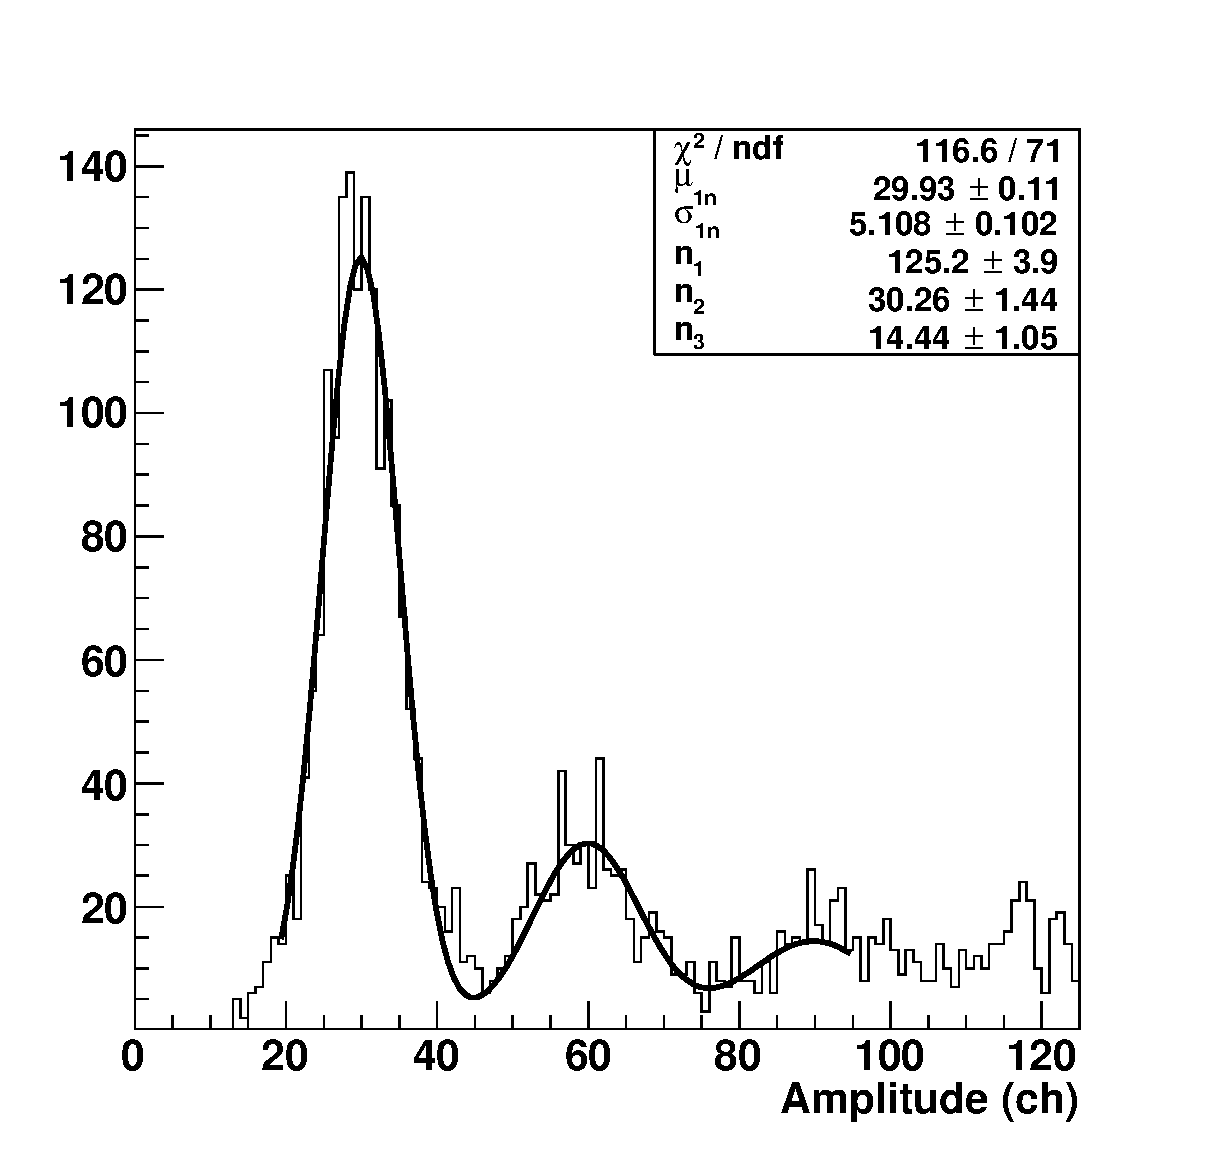
\includegraphics[viewport=0bp 0bp 569.4bp 736.111bp,clip,width=0.5\columnwidth]{zdc/fill_7457_dcmtnon_1n_resolution}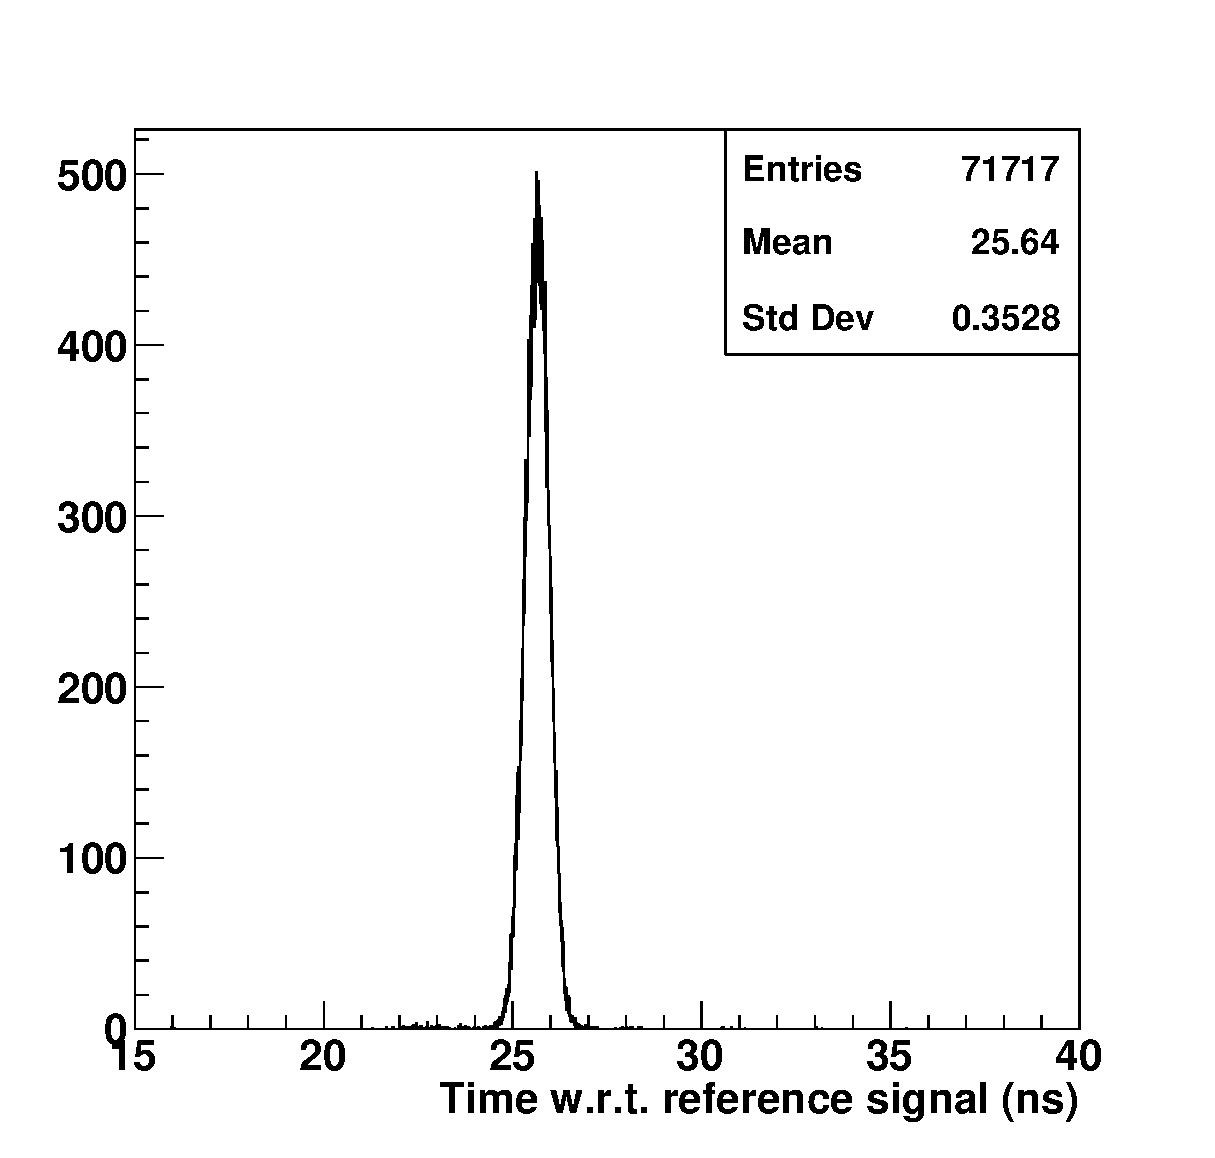
\includegraphics[viewport=0bp 0bp 569.4bp 736.111bp,clip,width=0.5\columnwidth]{zdc/run296549-part0-dcmtnon-d20181120-h1230_znctc_time}

    \caption{\label{fig:zdc-signals}Analysis of the performance of the digitizer during Pb-Pb 2018 data taking in the operating conditions chosen for RUN3. On the left plot: the lower part of the triggered spectrum of ZNC common photomultiplier in Pb-Pb collisions where the emission of a single $\SI{2.76}{\tera\electronvolt}$ neutron  and multiples are visible. The autotrigger algoritm effectively rejects pedestal events. On the right plot: the arrival time of ZNC common photomultiplier
    signals w.r.t. the reference ALICE L0 trigger signal.}
\end{figure}
    
    



\section{Mechanics and integration (Werner, Corrado; 5 p.)}
Beampipe, support structures, detector alignment, installation and maintenance


\section{Read-out and data processing (20p.)}
\subsection{O2 Overview: reconstruction workflow (PDP) (Andreas; 5 p.)}
(TF structure, …)
\subsection{CTP (David; 3p.)}
\subsection{CRU (Tivadar, Alex; 3 p.)}
\subsection{FLP (Pierre; 3p.)}
Here come the text for the O2 FLP project.
\subsection{EPN (Volker; 3p.)}
\subsection{Grid computing (Andreas; 3 p.)}


\section{Conclusions (Werner, Alex, Marco, Jochen; 5 p.)}
\subsection{Prospects for Run 3 + 4 (expected performance)}


\cleardoublepage
%%%%% acknowledgements - handled by EB chairs
\newenvironment{acknowledgement}{\relax}{\relax}
\begin{acknowledgement}
\section*{Acknowledgements}
% add specific acknowledgements here
% ...but please don't remove the line below: funding agencies
% will be acknowledged with a custom tex file handled by EB chairs after Collab Round 2
%\input{acknowledgements.tex}
\end{acknowledgement}

%%%%%%%% Bibliography
\bibliographystyle{utphys}   % Remember we use title in the biblio
\bibliography{bibliography}
%\input {bibliography.tex}

%%%%%%%%%%%%%%%%%%%%%%%%%%%%%%%%
% Appendices: yours (if any) + authorlist
%%%%%%%%%%%%%%%%%%%%%%%%%%%%%%%%
\newpage
\appendix

%
%\input{} % put your appendices here (if any)
%

%%%%% Authorlist - please do not touch: handled by EB chairs
\section{The ALICE Collaboration}
\label{app:collab}
%\input{authorlist-preprint.tex}
\end{document}
